% =====================================================================
%  Propuesta de proyecto — Software de monitoreo de salud autónomo
%  Compilar con: xelatex propuesta.tex  (dos veces)
% =====================================================================
\documentclass[11pt,a4paper]{article}

% ---------- Idioma y tipografía ----------
\usepackage{fontspec}
\usepackage{babel}
\babelprovide[import, main]{spanish}
\setmainfont{TeX Gyre Pagella}
\setsansfont{Inter}
\newfontfamily\display{Inter Display}
\newfontfamily\mono{DejaVu Sans Mono}[Scale=0.85]
\linespread{1.12}

% ---------- Página y color ----------
\usepackage[a4paper, top=2.6cm, bottom=2.4cm, left=2.5cm, right=2.5cm, headheight=14pt]{geometry}
\usepackage{xcolor}
\definecolor{navy}{HTML}{0B1F3A}
\definecolor{navy2}{HTML}{14325C}
\definecolor{mars}{HTML}{C1440E}
\definecolor{marslight}{HTML}{F7E4DA}
\definecolor{teal}{HTML}{1F7A8C}
\definecolor{teallight}{HTML}{DDEFF2}
\definecolor{ink}{HTML}{1E2430}
\definecolor{muted}{HTML}{5B6573}
\definecolor{rule}{HTML}{D5DAE1}
\definecolor{paper}{HTML}{F5F7FA}
\definecolor{ok}{HTML}{2E8B57}
\definecolor{warn}{HTML}{D9A21B}
\color{ink}

% ---------- Paquetes ----------
\usepackage{tikz}
\usetikzlibrary{positioning, arrows.meta, shapes.geometric, calc, fit, backgrounds, decorations.pathreplacing}
\usepackage[most]{tcolorbox}
\usepackage{titlesec}
\usepackage{enumitem}
\usepackage{tabularx, booktabs, array, colortbl}
\renewcommand{\tabularxcolumn}[1]{>{\raggedright\arraybackslash}p{#1}}
\usepackage{fancyhdr}
\usepackage{microtype}
\usepackage[hidelinks]{hyperref}
\hypersetup{colorlinks=true, linkcolor=navy2, urlcolor=teal}
\usepackage{xurl}
\usepackage{multicol}
\usepackage{xltabular}
\usepackage{pifont}
\usepackage{amssymb}
\usepackage[autostyle]{csquotes}

% ---------- Títulos ----------
\titleformat{\section}{\sffamily\Large\bfseries\color{navy}}{%
  \makebox[0pt][r]{\color{mars}\thesection\hspace{0.6em}}}{0pt}{}
\titlespacing*{\section}{0pt}{1.6em}{0.7em}
\titleformat{\subsection}{\sffamily\large\bfseries\color{navy2}}{}{0pt}{}
\titlespacing*{\subsection}{0pt}{1.1em}{0.4em}
\titleformat{\subsubsection}{\sffamily\normalsize\bfseries\color{teal}}{}{0pt}{}
\setlength{\parskip}{0.55em}
\setlength{\parindent}{0pt}
\setlength{\emergencystretch}{3em}
\tolerance=2000

% ---------- Encabezado y pie ----------
\pagestyle{fancy}
\fancyhf{}
\renewcommand{\headrulewidth}{0pt}
\fancyhead[L]{\sffamily\footnotesize\color{muted}Monitoreo de salud autónomo}
\fancyhead[R]{\sffamily\footnotesize\color{muted}\leftmark}
\fancyfoot[R]{\sffamily\footnotesize\color{navy}\bfseries\thepage}
\fancyfoot[L]{\sffamily\footnotesize\color{muted}Propuesta de proyecto · NASA Space Apps Challenge}
\renewcommand{\sectionmark}[1]{\markboth{#1}{}}

% ---------- Listas ----------
\setlist{itemsep=0.25em, topsep=0.3em}
\setlist[itemize]{label={\color{mars}\small$\blacktriangleright$}, leftmargin=1.4em}
\setlist[enumerate]{label={\sffamily\bfseries\color{teal}\arabic*.}, leftmargin=1.6em}

% ---------- Cajas ----------
\newtcolorbox{keybox}[1]{enhanced, breakable, colback=paper, colframe=navy,
  boxrule=0pt, leftrule=3.5pt, arc=2pt, left=10pt, right=10pt, top=8pt, bottom=8pt,
  title={\sffamily\bfseries #1}, coltitle=navy, colbacktitle=paper,
  attach title to upper, after title={\par\smallskip}}
\newtcolorbox{questionbox}{enhanced, colback=navy, colframe=navy, coltext=white,
  arc=3pt, boxrule=0pt, left=14pt, right=14pt, top=12pt, bottom=12pt,
  overlay={\node[anchor=north east, font=\display\bfseries\fontsize{54}{54}\selectfont,
    text=mars, opacity=0.9] at ([xshift=-8pt, yshift=6pt]frame.north east) {?};}}
\newtcolorbox{notebox}{enhanced, colback=marslight, colframe=marslight, arc=2pt,
  boxrule=0pt, left=10pt, right=10pt, top=6pt, bottom=6pt, fontupper=\small}

% Tarjeta de cifra
\newcommand{\statcard}[3]{%
  \begin{tcolorbox}[enhanced, width=\linewidth, colback=white, colframe=rule, boxrule=0.6pt,
    arc=3pt, left=8pt, right=8pt, top=7pt, bottom=7pt, height=3.15cm, valign=top]
    {\display\bfseries\fontsize{24}{26}\selectfont\color{#1}#2}\par\vspace{3pt}
    {\sffamily\footnotesize\raggedright\color{ink}#3\par}
  \end{tcolorbox}}

% Página divisoria de parte
\newcommand{\partpage}[3]{%
  \clearpage\thispagestyle{empty}
  \begin{tikzpicture}[remember picture, overlay]
    \fill[navy] (current page.north west) rectangle (current page.south east);
    \foreach \i in {1,...,140}{
      \pgfmathsetmacro{\x}{rnd*21}\pgfmathsetmacro{\y}{rnd*29.7}\pgfmathsetmacro{\r}{0.2+rnd*0.9}
      \fill[white, opacity=0.25+0.5*rnd] ($(current page.south west)+(\x,\y)$) circle (\r pt);}
    \draw[white, opacity=0.12, line width=0.6pt] ($(current page.south east)+(-2,6)$) circle (9cm);
    \shade[ball color=mars, opacity=0.95] ($(current page.south east)+(-2.2,4.4)$) circle (2.1cm);
    \node[anchor=north west, text width=15cm, align=left] at ($(current page.north west)+(2.5,-8.5)$) {%
      {\sffamily\bfseries\color{mars}\Large #1}\par\vspace{0.6cm}
      {\display\bfseries\color{white}\fontsize{38}{44}\selectfont #2}\par\vspace{0.8cm}
      {\sffamily\color{white!80!navy}\large #3}};
  \end{tikzpicture}
  \clearpage}

\pgfmathsetseed{20261106}

% =====================================================================
\begin{document}

% ------------------------------ PORTADA ------------------------------
\thispagestyle{empty}
\begin{tikzpicture}[remember picture, overlay]
  \fill[navy] (current page.north west) rectangle (current page.south east);
  \foreach \i in {1,...,220}{
    \pgfmathsetmacro{\x}{rnd*21}\pgfmathsetmacro{\y}{rnd*29.7}\pgfmathsetmacro{\r}{0.2+rnd*1.0}
    \fill[white, opacity=0.2+0.6*rnd] ($(current page.south west)+(\x,\y)$) circle (\r pt);}
  % órbita Tierra–Marte
  \draw[white, opacity=0.18, line width=0.7pt] ($(current page.south west)+(10.5,5.5)$) ellipse (13cm and 5.2cm);
  \draw[mars, opacity=0.8, line width=1.1pt, dashed, -{Stealth[length=7pt]}]
     ($(current page.south west)+(2.2,3.2)$) .. controls +(5,4.5) and +(-6,1.5) .. ($(current page.south west)+(16.4,8.6)$);
  \shade[ball color=teal!70!white, opacity=0.95] ($(current page.south west)+(2.2,3.2)$) circle (0.85cm);
  \shade[ball color=mars, opacity=0.97] ($(current page.south west)+(17.4,9.1)$) circle (1.55cm);
  \node[font=\sffamily\scriptsize, text=white!70!navy] at ($(current page.south west)+(2.2,1.9)$) {Tierra};
  \node[font=\sffamily\scriptsize, text=white!70!navy] at ($(current page.south west)+(17.4,7.1)$) {Marte};
  \node[font=\sffamily\scriptsize, text=mars!60!white, rotate=17] at ($(current page.south west)+(9.6,7.1)$) {hasta 20 min de retraso por sentido};
  % Texto
  \node[anchor=north west, text width=16cm, align=left] at ($(current page.north west)+(2.4,-3.2)$) {%
    {\sffamily\bfseries\color{mars}\large PROPUESTA DE PROYECTO · NASA SPACE APPS CHALLENGE}\par\vspace{0.9cm}
    {\display\bfseries\color{white}\fontsize{36}{42}\selectfont Monitoreo de salud\\[2pt] autónomo para misiones\\[2pt] de larga duración}\par\vspace{0.8cm}
    {\sffamily\color{white!82!navy}\Large Un software que compara a cada astronauta\\ consigo mismo y le dice qué hacer, sin depender de la Tierra}\par\vspace{1.4cm}
    \begin{tikzpicture}
      \foreach \t/\c [count=\k] in {Contexto y problema/mars, Objetivos/mars, Arquitectura/teal, Herramientas y funciones/teal}{
        \node[anchor=west, font=\sffamily\small, text=white, fill=\c, rounded corners=2pt, inner sep=4pt]
          at (0, -\k*0.62) {\bfseries\k\quad\t};}
    \end{tikzpicture}};
  \node[anchor=south west, text width=16cm, align=left] at ($(current page.south west)+(2.4,12.6)$) {%
    {\sffamily\small\color{white!75!navy}Noviembre de 2026}};
\end{tikzpicture}
\clearpage

% ------------------------------ RESUMEN ------------------------------
\section*{Resumen de la propuesta}
\markboth{Resumen}{}

En una misión a Marte, la señal tarda hasta 20 minutos en llegar a la Tierra y la tripulación no puede volver ante una emergencia. Mientras tanto, el cuerpo cambia en silencio: los huesos pierden densidad, la vista se altera, el sistema inmune se debilita y el aislamiento afecta el sueño y el ánimo. Proponemos un \textbf{software de monitoreo de salud que funciona a bordo, sin conexión}, aprende la línea base de cada astronauta y le avisa, con lenguaje claro, qué está cambiando y qué hacer.

\vspace{0.4em}
\begin{multicols}{2}
\begin{keybox}{Parte I · El problema}
\begin{itemize}[leftmargin=1.1em]
  \item Evidencia real de la NASA sobre seis sistemas del cuerpo.
  \item La brecha: no hay médico en tiempo real.
  \item Pregunta de investigación y objetivos.
\end{itemize}
\end{keybox}
\columnbreak
\begin{keybox}{Parte II · La solución}
\begin{itemize}[leftmargin=1.1em]
  \item Arquitectura en cinco capas, todo a bordo.
  \item Herramientas: Python, FastAPI, Vue (PWA), SQLite.
  \item Diez funciones, de la medición a la recomendación.
\end{itemize}
\end{keybox}
\end{multicols}

\vspace{0.2em}
\begin{center}
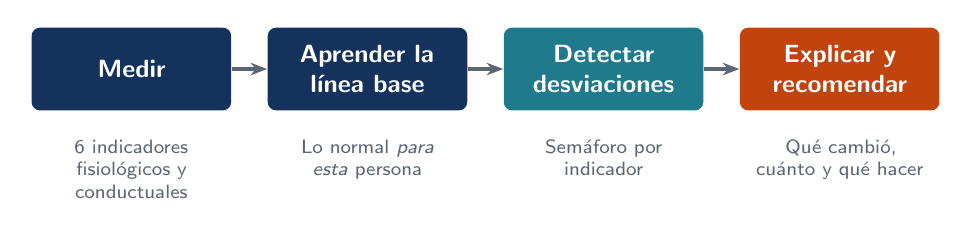
\begin{tikzpicture}[
  stage/.style={rectangle, rounded corners=3pt, fill=#1, text=white, font=\sffamily\small\bfseries,
                minimum height=1.05cm, text width=2.3cm, align=center},
  arr/.style={-{Stealth[length=6pt]}, line width=1.1pt, color=muted}]
  \node[stage=navy2] (a) {Medir};
  \node[stage=navy2, right=0.45cm of a] (b) {Aprender la línea base};
  \node[stage=teal, right=0.45cm of b] (c) {Detectar desviaciones};
  \node[stage=mars, right=0.45cm of c] (d) {Explicar y recomendar};
  \draw[arr] (a) -- (b); \draw[arr] (b) -- (c); \draw[arr] (c) -- (d);
  \node[below=0.25cm of a, font=\sffamily\scriptsize, text=muted, text width=2.4cm, align=center] {6 indicadores fisiológicos y conductuales};
  \node[below=0.25cm of b, font=\sffamily\scriptsize, text=muted, text width=2.4cm, align=center] {Lo normal \emph{para esta} persona};
  \node[below=0.25cm of c, font=\sffamily\scriptsize, text=muted, text width=2.4cm, align=center] {Semáforo por indicador};
  \node[below=0.25cm of d, font=\sffamily\scriptsize, text=muted, text width=2.4cm, align=center] {Qué cambió, cuánto y qué hacer};
\end{tikzpicture}
\end{center}

% =====================================================================
\partpage{PARTE I}{Contexto, problema\\ y objetivos}{Lo que dice la literatura científica sobre la salud\\ de los astronautas en misiones de larga duración}

\section{Contexto}

Las misiones tripuladas de larga duración, como un viaje a Marte de aproximadamente tres años entre tránsito y estancia en superficie, representan el mayor desafío para la salud humana en la historia de la exploración espacial. El Human Research Program (HRP) de la NASA agrupa las amenazas de estas misiones en cinco peligros, resumidos en el acrónimo RIDGE (NASA, s.f.):

\begin{center}

\begin{tikzpicture}[
  r/.style={circle, minimum size=1.35cm, fill=navy, text=white, font=\display\bfseries\Large},
  l/.style={font=\sffamily\scriptsize, text width=2.35cm, align=center, text=ink}]
  \foreach \L/\T [count=\i] in {R/Radiación espacial, I/Aislamiento y confinamiento, D/Distancia a la Tierra, G/Gravedad alterada, E/Ambiente cerrado y hostil}{
    \node[r] (n\i) at (\i*2.85, 0) {\L};
    \node[l, below=0.18cm of n\i] {\T};}
\end{tikzpicture}
\end{center}

De estos cinco peligros se derivan más de 30 riesgos para la salud documentados por el HRP; los clasificados como \enquote{rojos} tienen la máxima prioridad porque combinan una alta probabilidad de ocurrencia con un impacto severo en la salud, el desempeño durante la misión y la calidad de vida a largo plazo (Patel et al., 2020). Sin embargo, casi toda la evidencia disponible en humanos proviene de misiones de cuatro a doce meses en la Estación Espacial Internacional (ISS), donde la tripulación cuenta con comunicación casi inmediata con la Tierra y puede regresar en pocas horas ante una emergencia, condiciones que no existirán en el espacio profundo.

\section{Efectos documentados en la salud}

La evidencia científica muestra que los vuelos de larga duración alteran prácticamente todos los sistemas del organismo. Las cifras clave son las siguientes:

\vspace{0.3em}
\noindent
\begin{minipage}[t]{0.235\linewidth}\statcard{mars}{1–1,5\,\%}{de densidad mineral ósea perdida \textbf{por mes} (NASA HRP, 2017)}\end{minipage}\hfill
\begin{minipage}[t]{0.235\linewidth}\statcard{mars}{$\approx$66\,\%}{de astronautas con signos tempranos de SANS (NASA, 2023)}\end{minipage}\hfill
\begin{minipage}[t]{0.235\linewidth}\statcard{teal}{$\approx$50\,\%}{con reactivación del virus varicela-zóster en la ISS (Crucian et al., s.f.)}\end{minipage}\hfill
\begin{minipage}[t]{0.235\linewidth}\statcard{teal}{93\,\%}{de semanas con síntomas depresivos en un tripulante de Mars-520 (Basner et al., 2014)}\end{minipage}

\subsection{Evidencia integral: el NASA Twins Study}
El estudio más completo hasta la fecha comparó durante 340 días al astronauta Scott Kelly, a bordo de la ISS, con su gemelo idéntico en Tierra. Encontró cambios metabólicos, alteraciones en la metilación del ADN de células inmunes, modificaciones en la microbiota intestinal, un engrosamiento de la pared de la arteria carótida que persistió durante toda la misión y una disminución de la velocidad y precisión cognitiva después del vuelo (Garrett-Bakelman et al., 2019). Aunque la mayoría de estos cambios se revirtió tras el regreso, no todos lo hicieron.

\subsection{Sistema óseo}
En ausencia de gravedad, los astronautas pierden entre el 1\,\% y el 1,5\,\% de su densidad mineral ósea por mes en los huesos que soportan peso (NASA Human Research Program, 2017). En tripulantes de la ISS con misiones de cuatro a seis meses, la pérdida fue de 0,9\,\% mensual en la columna y de 1,4\,\% a 1,5\,\% mensual en la cadera (Lang et al., 2004). Se desconoce si esta pérdida se estabiliza o continúa en misiones de más de seis meses.

\subsection{Sistema neuro-ocular (SANS)}
Aproximadamente el 66\,\% de los astronautas de larga duración presenta los primeros signos del síndrome neuro-ocular asociado al vuelo espacial, y el edema del disco óptico aparece en cerca del 64\,\% de los casos (NASA, 2023). Aún no se sabe qué gravedad o duración de estos signos puede producir daños permanentes en la visión.

\subsection{Sistema inmune}
Durante misiones de seis meses en la ISS se observan cambios en la distribución de leucocitos, menor función de los linfocitos T y reactivación de herpesvirus latentes (Crucian et al., s.f.). Estas alteraciones se asocian con niveles elevados de cortisol y no se resuelven a lo largo de la misión (Crucian et al., 2018).

\subsection{Radiación}
Se estima que una misión a Marte de unos tres años expondría a cada astronauta a una dosis de 300 a 450\,mGy, con mayor riesgo de cáncer, enfermedad cardiovascular y deterioro cognitivo (Patel et al., 2020).

\subsection{Salud conductual}
Es uno de los riesgos más difíciles de mitigar. En Mars-520, una simulación terrestre de 520 días de aislamiento, un tripulante desarrolló insomnio crónico con fallas de atención y otro reportó síntomas depresivos en el 93\,\% de las semanas; en cambio, dos tripulantes no mostraron ninguna alteración (Basner et al., 2014).

\begin{keybox}{Dos conclusiones que guían el diseño}
\begin{enumerate}
  \item \textbf{Cada persona responde distinto.} Los umbrales poblacionales fijos resultan insuficientes: hay que comparar a cada astronauta con su propia línea base.
  \item \textbf{Los sistemas interactúan.} El estrés y el sueño deficiente elevan el cortisol, lo que a su vez debilita la respuesta inmune (Crucian et al., 2018). Hay que mirar los indicadores en conjunto.
\end{enumerate}
\end{keybox}

\section{La brecha: autonomía médica sin apoyo en tiempo real}

El modelo médico actual no es trasladable a Marte. En la ISS, la cercanía a la Tierra permite comunicación casi instantánea, telemetría médica continua y evacuación rápida, en un esquema de \enquote{estabilizar y regresar}; por ello, los astronautas ejercen una autonomía clínica limitada (Canadian Space Agency [CSA], 2025). En una misión a Marte, la señal puede tardar hasta 20 minutos en cada sentido, lo que hace inviable la telemedicina en tiempo real (CSA, 2025), y existen periodos de apagón total de comunicaciones (International Astronautical Congress [IAC], 2021).

\begin{center}
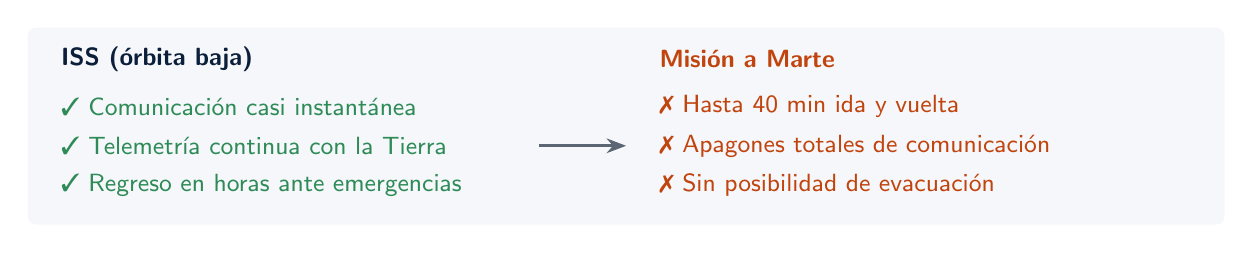
\begin{tikzpicture}[font=\sffamily\small]
  \fill[paper, rounded corners=3pt] (-0.3,-1.15) rectangle (14.9,1.35);
  \node[font=\sffamily\bfseries\small, text=navy, anchor=west] at (0,0.95) {ISS (órbita baja)};
  \node[font=\sffamily\bfseries\small, text=mars, anchor=west] at (7.6,0.95) {Misión a Marte};
  \foreach \t/\y in {Comunicación casi instantánea/0.35, Telemetría continua con la Tierra/-0.15, Regreso en horas ante emergencias/-0.65}
    \node[anchor=west, text=ink] at (0,\y) {\color{ok}\ding{51}\ \t};
  \foreach \t/\y in {Hasta 40 min ida y vuelta/0.35, Apagones totales de comunicación/-0.15, Sin posibilidad de evacuación/-0.65}
    \node[anchor=west, text=ink] at (7.6,\y) {\color{mars}\ding{55}\ \t};
  \draw[-{Stealth[length=7pt]}, line width=1.2pt, muted] (6.2,-0.15) -- (7.3,-0.15);
\end{tikzpicture}
\end{center}

Ante esta realidad, la medicina espacial pasa de una atención dependiente de la Tierra a las \textbf{operaciones médicas independientes de la Tierra} (EIMO), en las que la tripulación asume progresivamente el diagnóstico y la toma de decisiones (CSA, 2025). El propio astronauta debe detectar en sí mismo cambios lentos y silenciosos, como la pérdida ósea o el SANS, y cambios subjetivos difíciles de reconocer desde dentro, como la fatiga, el ánimo o el deterioro cognitivo. \textbf{Los datos para hacerlo existen, pero están dispersos en sensores, pruebas y cuestionarios que no se integran en una lectura única, comparada con la línea base de cada persona y traducida en una acción concreta.}

\section{Planteamiento del problema}

\begin{keybox}{Enunciado del problema}
En las misiones de larga duración fuera de la órbita baja terrestre, los astronautas experimentan cambios óseos, neuro-oculares, inmunes, cardiovasculares y conductuales bien documentados, que avanzan de forma gradual y varían considerablemente entre individuos (Basner et al., 2014; Garrett-Bakelman et al., 2019; Patel et al., 2020). Con retrasos de comunicación de hasta 20 minutos por sentido, la tripulación no puede depender del equipo médico en Tierra para detectarlos a tiempo (CSA, 2025). \textbf{Actualmente no existe una herramienta que reúna los indicadores de salud de cada astronauta, los compare con su propia línea base y le indique, en un lenguaje claro, qué está cambiando y qué acciones tomar.}
\end{keybox}

\vspace{0.4em}
\begin{questionbox}
{\sffamily\bfseries\small\color{mars!70!white} PREGUNTA DE INVESTIGACIÓN}\par\vspace{0.4em}
\begin{minipage}{0.86\linewidth}
\large ¿De qué manera puede desarrollarse un software de monitoreo de salud que, a partir de la línea base individual construida con datos abiertos de la NASA (OSDR, Inspiration4) y del análogo Mars-520, integre indicadores fisiológicos (frecuencia cardíaca, variabilidad de la frecuencia cardíaca, sueño y dosis de radiación acumulada) y conductuales (vigilancia psicomotora y estado de ánimo) para que un astronauta detecte desviaciones en su salud y decida qué acciones tomar durante una misión a Marte, sin depender de la comunicación en tiempo real con la Tierra?
\end{minipage}
\end{questionbox}

\begin{notebox}
\textbf{Alcance para el hackatón.} Se limita a indicadores que pueden medirse a bordo sin equipo de laboratorio: signos vitales, sueño, ejercicio, dosis de radiación, pruebas cognitivas breves y autorreportes. \textbf{El sistema no pretende diagnosticar enfermedades, sino servir como apoyo a la toma de decisiones.}
\end{notebox}

\section{Objetivos}

\begin{tcolorbox}[enhanced, colback=teallight, colframe=teallight, arc=3pt, boxrule=0pt, left=12pt, right=12pt, top=10pt, bottom=10pt]
{\sffamily\bfseries\color{teal}OBJETIVO GENERAL}\par\vspace{0.3em}
Desarrollar un software de monitoreo de salud para astronautas que funcione sin conexión con la Tierra, integre indicadores fisiológicos y conductuales, detecte desviaciones respecto a la línea base de cada tripulante y recomiende acciones basadas en evidencia, utilizando datos abiertos de la NASA (OSDR, Inspiration4) y del análogo Mars-520 para su construcción y validación.
\end{tcolorbox}

{\sffamily\bfseries\color{navy}Objetivos específicos}
\begin{enumerate}
  \item Definir los seis indicadores a vigilar a partir de la literatura de la NASA, con su frecuencia de medición y su rango de referencia.
  \item Combinar datos reales con datos simulados que reproduzcan una misión a Marte con desviaciones de salud conocidas.
  \item Diseñar un módulo para el cálculo de la línea base de cada astronauta y la detección de desviaciones en cada indicador.
  \item Implementar alertas que expliquen qué indicador cambió, cuánto y qué hacer, sin necesitar conexión con la Tierra.
  \item Evaluar el software en una misión simulada y compararlo con umbrales fijos, iguales para todos, midiendo cuántos días antes detecta los cambios, cuántos detecta (sensibilidad) y cuántas falsas alarmas da.
\end{enumerate}

\section{Justificación}

Este proyecto responde directamente a los riesgos de mayor prioridad identificados por el HRP de la NASA y a la necesidad de autonomía médica para misiones a Marte (CSA, 2025; Patel et al., 2020). Su principal aporte es la \textbf{detección temprana}: cambios como la pérdida ósea o el SANS son graduales, por lo que vigilarlos de forma continua permite aplicar contramedidas, como ajustes en el ejercicio, la dieta o el sueño, antes de que se produzca un daño significativo. Además, la variabilidad entre individuos observada en Mars-520 indica que los umbrales poblacionales fijos no son suficientes (Basner et al., 2014). Por último, la solución tiene \textbf{aplicación en la Tierra}: puede servir a personal en bases antárticas, submarinos o plataformas petroleras, y a comunidades rurales sin médico, como las zonas aisladas de los Andes y la Amazonía.

% =====================================================================
\partpage{PARTE II}{Arquitectura,\\ herramientas y funciones}{Cómo se construye el software: capas, tecnologías\\ y lo que podrá hacer el astronauta}

\section{Punto de partida: software existente}

Ningún sistema actual reúne indicadores fisiológicos y conductuales, los compara con la línea base de cada astronauta y recomienda acciones sin depender de la Tierra. Pero varios resuelven partes del problema, y de ellos tomamos ideas y código:

\begin{center}
\small
\renewcommand{\arraystretch}{1.35}
\begin{tabularx}{\linewidth}{
>{\raggedright\arraybackslash\leavevmode\sffamily\bfseries\color{navy}}p{3.1cm} X X}
\toprule
{\sffamily\color{muted}Sistema} & \leavevmode{\sffamily\bfseries\color{muted}Qué resuelve} & \leavevmode{\sffamily\bfseries\color{muted}Qué tomamos} \\
\midrule
Astroskin (CSA) & Camiseta con sensores en la ISS desde 2019; los datos se analizan en la Tierra (Canadian Space Agency, s.f.) & Indicadores y modelo de datos del sensor \\
Reaction Self-Test (NASA) & Prueba de reacción que compara al astronauta consigo mismo, solo para fatiga (NASA, 2013) & Diseño del módulo cognitivo PVT-B \\
Clinical Decision Support (NASA) & Apoyo a decisiones en emergencias, no seguimiento continuo (NASA, 2020) & Formato de recomendación \\
\rowcolor{teallight}AnomalyDetect (Stanford) & Línea base personal y alertas por colores con datos de reloj inteligente; código abierto (Bogu, 2020; Mishra et al., 2020) & \textbf{Inspiración del método: línea base personal y semáforo} \\
RapidHRV & Cálculo de la variabilidad de la frecuencia cardíaca; código abierto (Kirk et al., 2022) & Mejora futura si se usan señales crudas de un sensor real \\
\bottomrule
\end{tabularx}
\end{center}

\begin{notebox}
\textbf{Prueba técnica ya realizada.} Actualizamos AnomalyDetect para Python 3.13 y lo ejecutamos con los datos de ejemplo del repositorio. Funciona: con 834 horas evaluadas de un usuario, marcó 7 días en rojo, 6 en amarillo y 27 en verde. Para el prototipo tomamos su lógica, pero la programamos de forma más sencilla con pandas y NumPy, la extendemos a seis indicadores y añadimos las recomendaciones.
\end{notebox}

\section{Arquitectura del software}

El software se organiza en \textbf{cinco capas} que funcionan \textbf{completamente a bordo}. La comunicación con la Tierra no es necesaria para operar: cuando hay enlace, solo se envía un resumen de forma diferida.

\begin{center}
\begin{tikzpicture}[
  font=\sffamily\small,
  layer/.style={rectangle, rounded corners=4pt, fill=#1, minimum width=13cm, minimum height=1.55cm},
  lab/.style={font=\sffamily\bfseries\small, text=white, anchor=west, text width=2.3cm},
  comp/.style={rectangle, rounded corners=2.5pt, fill=white, draw=none, font=\sffamily\scriptsize,
               text=ink, minimum height=0.9cm, text width=2.0cm, align=center, inner sep=2pt},
  flow/.style={-{Stealth[length=6pt]}, line width=1.2pt, color=mars}]
  % capas (de arriba hacia abajo)
  \node[layer=mars] (L5) at (0,0) {};
  \node[layer=teal] (L4) at (0,-2.0) {};
  \node[layer=navy2] (L3) at (0,-4.0) {};
  \node[layer=navy2!80!teal] (L2) at (0,-6.0) {};
  \node[layer=navy] (L1) at (0,-8.0) {};
  % etiquetas
  \node[lab] at ($(L5.west)+(0.25,0)$) {5 · Presentación};
  \node[lab] at ($(L4.west)+(0.25,0)$) {4 · Decisión};
  \node[lab] at ($(L3.west)+(0.25,0)$) {3 · Análisis};
  \node[lab] at ($(L2.west)+(0.25,0)$) {2 · Datos};
  \node[lab] at ($(L1.west)+(0.25,0)$) {1 · Adquisición};
  % componentes
  \def\cx{-2.55}
  \foreach \t [count=\i] in {Panel del astronauta, Vista del oficial médico, Prueba PVT-B y check-in diario, Reporte para la Tierra}
    \node[comp] at (\cx+\i*2.35-2.35, 0) {\t};
  \foreach \t [count=\i] in {Semáforo por indicador, Índice global de salud, Reglas de recomendación, Explicación de la alerta}
    \node[comp] at (\cx+\i*2.35-2.35, -2.0) {\t};
  \foreach \t [count=\i] in {Cálculo de indicadores diarios, Línea base individual, {Puntaje z por indicador}, Comparador con umbrales fijos}
    \node[comp] at (\cx+\i*2.35-2.35, -4.0) {\t};
  \foreach \t [count=\i] in {Ingesta y validación, Base de datos local (SQLite), Perfil por astronauta, Registro de eventos}
    \node[comp] at (\cx+\i*2.35-2.35, -6.0) {\t};
  \foreach \t [count=\i] in {{Wearable: FC, HRV y sueño}, Dosímetro personal, Tableta: PVT y ánimo, Simulador de misión}
    \node[comp] at (\cx+\i*2.35-2.35, -8.0) {\t};
  % flujo
  \foreach \a/\b in {L1/L2, L2/L3, L3/L4, L4/L5}
    \draw[flow] ($(\a.north east)+(-0.35,0.02)$) -- ($(\b.south east)+(-0.35,-0.02)$);
  % marco "a bordo"
  \begin{scope}[on background layer]
    \node[draw=muted, dashed, rounded corners=6pt, line width=0.7pt, inner sep=9pt, fit=(L1)(L5)] (onboard) {};
  \end{scope}
  \node[anchor=south west, font=\sffamily\scriptsize\bfseries, text=muted] at (onboard.north west) {A BORDO · FUNCIONA SIN CONEXIÓN};
  % Tierra
  \node[circle, shade, ball color=teal!70!white, minimum size=1.1cm, font=\sffamily\scriptsize\bfseries, text=white] (earth) at (8.05,0) {Tierra};
  \draw[-{Stealth[length=6pt]}, line width=1pt, muted, dashed] (L5.east) -- (earth.west);
  \node[below=0.15cm of earth, font=\sffamily\scriptsize, text=muted, text width=1.6cm, align=center] {envío diferido};
\end{tikzpicture}
\end{center}

\subsection{Descripción de las capas}

\begin{enumerate}
  \item \textbf{Adquisición.} Recoge los datos de los sensores: un wearable tipo Astroskin para frecuencia cardíaca, su variabilidad y el sueño; un dosímetro personal para la radiación; y la tableta para la prueba de vigilancia psicomotora y el autorreporte de ánimo. Para el hackatón, un \emph{simulador de misión} genera estos datos a partir de parámetros reales de la literatura.
  \item \textbf{Datos.} Valida y guarda todo en una base de datos local (SQLite), organizada por astronauta. Al no depender de un servidor externo, funciona sin conexión.
  \item \textbf{Análisis.} Es el núcleo científico. Con pandas y NumPy, resume cada indicador por día, calcula la línea base de cada persona con una ventana móvil de días anteriores y mide cuánto se aleja el valor de hoy de lo normal \emph{para esa persona}. En paralelo, aplica umbrales fijos para poder comparar ambos métodos.
  \item \textbf{Decisión.} Convierte cada anomalía en un semáforo (verde, amarillo o rojo) y en un índice global de salud. Un motor de reglas, construido a partir de la literatura de la NASA, asocia cada alerta con una recomendación concreta y explica por qué se generó.
  \item \textbf{Presentación.} Muestra al astronauta su estado de un vistazo, con tendencias y alertas; ofrece una vista para el oficial médico de la tripulación; y prepara un reporte que se envía a la Tierra cuando haya comunicación.
\end{enumerate}

\subsection{Indicadores que monitorea el sistema}

\begin{center}
\small
\renewcommand{\arraystretch}{1.18}
\begin{tabularx}{\linewidth}{
>{\raggedright\arraybackslash\leavevmode\sffamily\bfseries\color{navy}}p{3.2cm} X p{2.4cm} X}
\toprule
{\sffamily\color{muted}Indicador} & \leavevmode{\sffamily\bfseries\color{muted}Cómo se mide} & \leavevmode{\sffamily\bfseries\color{muted}Frecuencia} & \leavevmode{\sffamily\bfseries\color{muted}Riesgo asociado} \\
\midrule
FC en reposo & Wearable (ECG), cuando no hay movimiento & Continua & Cardiovascular, inmune \\
Variabilidad de la FC & Wearable (ECG), durante el sueño & Diaria & Estrés y recuperación \\
Sueño & Actigrafía del wearable & Diaria & Conductual, cognitivo, inmune \\
Dosis de radiación & Dosímetro personal & Continua & Cáncer, cardiovascular, cognitivo \\
Vigilancia psicomotora & Prueba PVT-B de 3 minutos en tableta & Diaria & Fatiga y rendimiento \\
Estado de ánimo & Autorreporte breve en tableta & Diaria & Salud conductual \\
\bottomrule
\end{tabularx}
\end{center}

\subsection{Cómo funciona la detección}

Para cada indicador, el sistema compara el valor de hoy con los días anteriores del mismo astronauta, siguiendo la misma idea de AnomalyDetect (Mishra et al., 2020) pero con un método más sencillo y fácil de explicar: el \textbf{puntaje z robusto}. Se toma una ventana de, por ejemplo, 14 días previos y se calcula:

\begin{equation*}
z = \frac{\text{valor de hoy} - \text{mediana de los días previos}}{1{,}4826 \times \text{desviación absoluta mediana}}
\end{equation*}

Se usa la mediana en lugar del promedio para que un día atípico no altere la línea base; el factor 1,4826 hace que el resultado se lea como desviaciones estándar. Según el indicador, importa si el valor sube (frecuencia cardíaca, fallos en la prueba PVT) o si baja (variabilidad, sueño, ánimo). El resultado se resume en tres niveles:

\begin{center}
\begin{tikzpicture}[font=\sffamily\small,
  lvl/.style={rectangle, rounded corners=3pt, minimum width=4.3cm, minimum height=1.35cm, text width=4cm, align=center, text=white}]
  \node[lvl, fill=ok] (g) {\textbf{VERDE} · $|z| < 2$\\[-1pt]{\scriptsize Dentro de su rango habitual}};
  \node[lvl, fill=warn, right=0.3cm of g] (y) {\textbf{AMARILLO} · $2 \le |z| < 3$\\[-1pt]{\scriptsize Desviación breve: vigilar y repetir}};
  \node[lvl, fill=mars, right=0.3cm of y] (r) {\textbf{ROJO} · $|z| \ge 3$\\[-1pt]{\scriptsize O 3 días seguidos en amarillo: actuar}};
\end{tikzpicture}
\end{center} Estos cortes son un punto de partida y se ajustarán con el simulador de misión.

Cada alerta responde tres preguntas: \textbf{qué indicador cambió}, \textbf{cuánto} (en desviaciones respecto a su línea base) y \textbf{qué hacer}. Ejemplos ilustrativos del motor de recomendaciones, que se ajustarán con la literatura durante el desarrollo:

\begin{center}
\small
\renewcommand{\arraystretch}{1.18}
\begin{tabularx}{\linewidth}{>{\raggedright\arraybackslash\sffamily}p{5.1cm} X}
\toprule
\leavevmode{\sffamily\bfseries\color{muted}Situación detectada} & \leavevmode{\sffamily\bfseries\color{muted}Recomendación al astronauta} \\
\midrule
{\color{mars}\textbf{Rojo}} · Vigilancia psicomotora baja tras dos noches de sueño corto & Posponer tareas críticas que exijan atención sostenida, priorizar el descanso y repetir la prueba al día siguiente \\
{\color{warn}\textbf{Amarillo}} · FC en reposo elevada y variabilidad baja & Reducir la intensidad del ejercicio del día, vigilar síntomas y revisar de nuevo en 24 horas \\
{\color{mars}\textbf{Rojo}} · Ánimo bajo durante varias semanas & Informar al oficial médico y activar los recursos de apoyo psicológico previstos en la misión \\
{\color{warn}\textbf{Amarillo}} · Dosis de radiación acumulada por encima de lo esperado & Revisar el tiempo fuera de las zonas más protegidas y seguir el procedimiento de la misión ante eventos solares \\
\bottomrule
\end{tabularx}
\end{center}


\section{Herramientas a utilizar}

Elegimos herramientas de código abierto, que el equipo ya conoce o puede aprender rápido, y que funcionan sin conexión. Para el análisis usamos solo pandas y NumPy: el método es sencillo, fácil de explicar y evita problemas de compatibilidad entre librerías.

{\small
\renewcommand{\arraystretch}{1.32}
\begin{xltabular}{\linewidth}{
>{\raggedright\arraybackslash\leavevmode\sffamily\bfseries\color{navy}}p{3.4cm} p{3.2cm} X}
\toprule
{\sffamily\color{muted}Herramienta} & \leavevmode{\sffamily\bfseries\color{muted}Capa} & \leavevmode{\sffamily\bfseries\color{muted}Para qué la usamos} \\
\midrule
\multicolumn{3}{l}{\cellcolor{paper}\sffamily\bfseries\scriptsize\color{teal} ANÁLISIS Y CIENCIA DE DATOS} \\
Python 3.12+ & Análisis & Lenguaje principal del motor de detección \\
pandas y NumPy & Datos, análisis & Series de tiempo por astronauta, línea base individual (ventana móvil), puntaje z, tendencias y semáforo \\
\multicolumn{3}{l}{\cellcolor{paper}\sffamily\bfseries\scriptsize\color{teal} BACKEND Y DATOS} \\
FastAPI & Datos, decisión & API local que conecta el motor con la interfaz \\
SQLite & Datos & Base de datos embebida, sin servidor, funciona sin conexión \\
\multicolumn{3}{l}{\cellcolor{paper}\sffamily\bfseries\scriptsize\color{teal} INTERFAZ} \\
Vue 3 + Vite & Presentación & Interfaz web del astronauta y del oficial médico \\
vite-plugin-pwa & Presentación & Convierte la interfaz en una app instalable que funciona sin conexión \\
Pinia y Vue Router & Presentación & Estado de la interfaz (alertas, astronauta seleccionado) y navegación entre vistas \\
Apache ECharts (vue-echarts) & Presentación & Gráficas de tendencias y semáforos \\
Prueba PVT-B (componente Vue) & Adquisición & Prueba de reacción de 3 minutos en la tableta \\
\multicolumn{3}{l}{\cellcolor{paper}\sffamily\bfseries\scriptsize\color{teal} DATOS REALES Y COLABORACIÓN} \\
NASA OSDR (API) & Adquisición & Datos de Inspiration4 y otras misiones \\
Docker & Despliegue & Ejecutar todo el sistema en un solo equipo, igual en cualquier computador \\
Git y GitHub & Equipo & Control de versiones y trabajo en paralelo \\
pytest & Validación & Pruebas automáticas del motor de detección \\
\bottomrule
\end{xltabular}}

\section{Funciones del software}

\begin{center}
\small
\renewcommand{\arraystretch}{1.22}
\begin{tabularx}{\linewidth}{>{\raggedright\arraybackslash\leavevmode\sffamily\bfseries\color{mars}}p{0.9cm} 
>{\raggedright\arraybackslash\leavevmode\sffamily\bfseries\color{navy}}p{4.0cm} X}
\toprule
{\sffamily\color{muted}N.º} & {\sffamily\color{muted}Función} & \leavevmode{\sffamily\bfseries\color{muted}Qué hace} \\
\midrule
F1 & Perfil del astronauta & Registra a cada tripulante y define su periodo inicial de línea base \\
F2 & Ingesta de datos & Recibe datos del wearable, el dosímetro o el simulador, y valida que estén completos \\
F3 & Prueba de vigilancia & Aplica la prueba PVT-B de 3 minutos y guarda tiempos de reacción y fallos \\
F4 & Check-in diario & Registra en menos de un minuto el ánimo y la calidad de sueño percibida \\
F5 & Línea base individual & Calcula lo normal para cada persona en cada indicador y la actualiza con el tiempo \\
F6 & Detección y semáforo & Detecta desviaciones y asigna verde, amarillo o rojo por indicador, más un índice global \\
F7 & Alertas explicables & Indica qué cambió, cuánto y qué hacer, con la fuente científica de la recomendación \\
F8 & Historial y tendencias & Muestra la evolución de cada indicador durante la misión \\
F9 & Simulador de misión & Genera una misión a Marte con desviaciones conocidas y apagones de comunicación, para validar el sistema \\
F10 & Reporte para la Tierra & Resume el estado de salud y lo deja listo para enviarse cuando haya enlace \\
\bottomrule
\end{tabularx}
\end{center}

\subsection{Validación}
Para responder a la pregunta de investigación, el simulador (F9) genera misiones con desviaciones conocidas. Se compara la detección basada en la línea base individual con la de umbrales fijos usando tres medidas: \textbf{cuántos días antes} detecta el cambio, \textbf{sensibilidad} (cuántos cambios detecta) y \textbf{tasa de falsas alarmas}.

\subsection{Pendientes por definir en equipo}
\begin{itemize}
  \item Confirmar qué conjuntos de datos exige o recomienda la página oficial del reto de NASA Space Apps.
  \item Definir el tamaño de la línea base y los cortes del semáforo: proponemos 14 días y $|z|$ de 2 y 3 (AnomalyDetect usa 31 días, que puede ser mucho al inicio de una misión).
  \item Repartir el trabajo entre análisis de datos, backend e interfaz.
  \item Mejora futura: registro de síntomas por voz, sin conexión.
\end{itemize}

% ------------------------------ REFERENCIAS ------------------------------
\clearpage
\section*{Referencias}
\markboth{Referencias}{}
\begingroup
\small
\setlength{\parindent}{-1.2em}\setlength{\leftskip}{1.2em}\setlength{\parskip}{0.3em}
\raggedright

Basner, M., Dinges, D. F., Mollicone, D. J., Savelev, I., et al. (2014). Psychological and behavioral changes during confinement in a 520-day simulated interplanetary mission to Mars. \emph{PLoS ONE, 9}(3), e93298. \url{https://doi.org/10.1371/journal.pone.0093298}

Bogu, G. K. (2020). \emph{AnomalyDetect} [Software]. GitHub. \url{https://github.com/gireeshkbogu/AnomalyDetect}

Canadian Space Agency. (s.f.). \emph{Bio-Monitor: Keeping an eye on astronauts' vital signs}. \url{https://www.asc-csa.gc.ca/eng/sciences/astroskin.asp}

Canadian Space Agency. (2025). \emph{Enabling Earth-independent medical operations: The CSA Connected Care Medical Module framework} (SpaceOps-2025, ID 92). \url{https://publications.spaceops.org/2025/download_by_id.php?id=0092}

Crucian, B. E., Choukèr, A., Simpson, R. J., Mehta, S., et al. (2018). Immune system dysregulation during spaceflight: Potential countermeasures for deep space exploration missions. \emph{Frontiers in Immunology, 9}, 1437. \url{https://doi.org/10.3389/fimmu.2018.01437}

Crucian, B. E., Stowe, R. P., Mehta, S., Uchakin, P., Quiriarte, H., Pierson, D., \& Sams, C. F. (s.f.). \emph{Immune system dysregulation and herpesvirus reactivation persist during long-duration spaceflight}. NASA Technical Reports Server. \url{https://ntrs.nasa.gov/citations/20100040666}

Garrett-Bakelman, F. E., Darshi, M., Green, S. J., Gur, R. C., et al. (2019). The NASA Twins Study: A multidimensional analysis of a year-long human spaceflight. \emph{Science, 364}(6436), eaau8650. \url{https://doi.org/10.1126/science.aau8650}

International Astronautical Congress. (2021). \emph{Autonomous medical operations for exploration class missions} (IAC-21,A1,4,7,x63236). \url{https://iafastro.directory/iac/paper/id/63236/}

Kirk, P. A., Davidson Bryan, A., Garfinkel, S. N., \& Robinson, O. J. (2022). RapidHRV: An open-source toolbox for extracting heart rate and heart rate variability. \emph{PeerJ, 10}, e13147. \url{https://doi.org/10.7717/peerj.13147}

Lang, T., LeBlanc, A., Evans, H., Lu, Y., Genant, H., \& Yu, A. (2004). Cortical and trabecular bone mineral loss from the spine and hip in long-duration spaceflight. \emph{Journal of Bone and Mineral Research, 19}(6), 1006–1012. \url{https://doi.org/10.1359/JBMR.040307}

Mishra, T., Wang, M., Metwally, A. A., Bogu, G. K., Brooks, A. W., Bahmani, A., Alavi, A., Celli, A., Higgs, E., Dagan-Rosenfeld, O., Fay, B., Kirkpatrick, S., Kellogg, R., Gibson, M., Wang, T., Hunting, E. M., Mamic, P., Ganz, A. B., Rolnik, B., \dots\ Snyder, M. P. (2020). Pre-symptomatic detection of COVID-19 from smartwatch data. \emph{Nature Biomedical Engineering, 4}(12), 1208–1220. \url{https://doi.org/10.1038/s41551-020-00640-6}

NASA. (s.f.). \emph{The human body in space}. \url{https://www.nasa.gov/humans-in-space/the-human-body-in-space/}

NASA. (2013). \emph{Health and medicine: Reaction Self-Test} (NASA Spinoff 2013). \url{https://spinoff.nasa.gov/Spinoff2013/hm_1.html}

NASA. (2020). \emph{Clinical decision support: Overview and update}. NASA Technical Reports Server. \url{https://ntrs.nasa.gov/citations/20205011448}

NASA. (2023). \emph{Spaceflight associated neuro-ocular syndrome (SANS): 2023 clinical update}. NASA Technical Reports Server. \url{https://ntrs.nasa.gov/citations/20220014606}

NASA Human Research Program. (2017). \emph{Evidence report: Risk of bone fracture due to spaceflight-induced changes to bone}. NASA Technical Reports Server. \url{https://ntrs.nasa.gov/citations/20170004597}

Patel, Z. S., Brunstetter, T. J., Tarver, W. J., Whitmire, A. M., et al. (2020). Red risks for a journey to the red planet: The highest priority human health risks for a mission to Mars. \emph{npj Microgravity, 6}, 33. \url{https://doi.org/10.1038/s41526-020-00124-6}

\endgroup
\end{document}
